An natural point to start using pgfplots is the axis-environment. We begin with the following simple example, which generates \cref{fig:simplepgfexample1}.

\verbatiminput{../src/figures/simplepgfexample1.tex}

\begin{figure}[h]
	\centering
	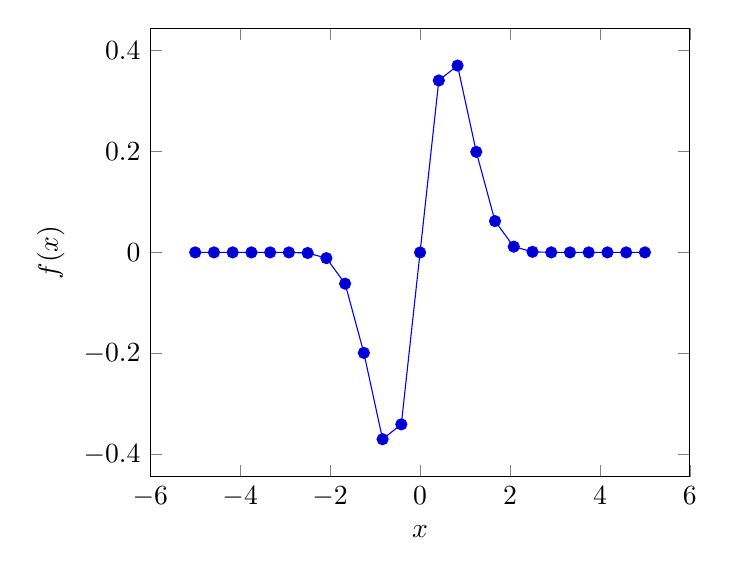
\begin{tikzpicture}
	\begin{axis}[
		xlabel=$x$, ylabel={$f(x)$},
		]
		\addplot {exp(-x^2)*sin(deg(x))};
	\end{axis}
\end{tikzpicture}
	\caption{This is fine for a start.}
	\label{fig:simplepgfexample1}
\end{figure}
\clearpage
Of course, we still want to improve this in many ways:

%\verbatiminput{../src/figures/simplepgfexample2.tex}

\begin{figure}[h]
	\centering
	\begin{tikzpicture}
	\begin{axis}[
		axis lines=center,
		width=\textwidth, height=\textwidth/\goldenratio,
		xlabel=$x$, ylabel={$f(x)$},
		grid=both,
		ymax=1.1,
		ymin=-1.1,
		]
		\addplot[
			domain=-3.2:3.2,
			samples=101, 
			line width=3,
			\colorforcurvesi]
			{exp(-x^2)*sin(deg(4*x))};
	\end{axis}
\end{tikzpicture}
	\caption{This one is a little more sophisticated.}
	\label{fig:simplepgfexample2}
\end{figure}

Now lets go for several functions:

%\verbatiminput{../src/figures/simplepgfexample3.tex}

\begin{figure*}[h]
\centering
\begin{tikzpicture}
	\begin{axis}[
		axis lines=center,
		width=\textwidth, height=\textwidth/\goldenratio,
		xlabel=$x$, ylabel={$y$},
		grid=both,
		ymax=1.4,
		ymin=-1,
		ytickmin=-0.5,
		ytickmax=1,
		legend style={draw=none,anchor=north east, at={(1,1)}},
		]
		\addplot[
		domain=-3.2:3.2,
		samples=101, 
		line width=3,
		\colorforcurvesv]
		{exp(-(x+1)^2)*sin(deg(3*(x+1)))};
		\addlegendentry{$g(x) = \euler^{-(x+1)^2}\sin\left(3(x+1)\right)$}
		\addplot[
		domain=-3.2:3.2,
		samples=101, 
		line width=3,
		\colorforcurvesi]
		{exp(-(x-1)^2)*sin(deg(4*(x-1)))};
		\addlegendentry{$f(x) = \euler^{-(x-1)^2}\sin\left(4(x-1)\right)$}
	\end{axis}
\end{tikzpicture}
\caption{This one is a little more sophisticated.}
\label{fig:simplepgfexample3}
\end{figure*}
\clearpage
Regarding marks and axis and grids see \cref{fig:discretization}.

\begin{figure*}
	\centering
	
\def\myplotxdist{8}
\def\myplotydist{7}
\begin{tikzpicture}
	\def\thefunction{(2.5 + x^8 + cos(deg(5*pi*x)) + cos(deg(6*pi*x)) + sin(deg(3*pi*x)))*exp(-x*x*2)*0.19}
	\def\myxmin{0}
	\def\myxmax{1}
	\def\myymin{0}
	\def\myymax{1}
	\def\mynsamples{30}
	\def\sampletimestep{(\myxmax - \myxmin)/(\mynsamples-1)}
	\def\mycolor{\colorforcurvesi}
	\def\mycolorii{\colorforcurvesii}
	\def\nquantsteps{30}
	\def\quantizeres{1/(\nquantsteps)}
	\def\mygridcolor{gray!20}
	\node (orig) at (0,0) {};
	\node[anchor=center] (conti) at (0,0) {
		\begin{tikzpicture}
			\begin{axis}[
				xmin=\myxmin,xmax=\myxmax,
				ymin=\myymin,ymax=\myymax,
				xlabel= $t  \in \realnumbers$,
				ylabel=$f(t) \in \realnumbers$,	
				xtick=\empty, 
				ytick=\empty, 
				]
				\addplot[domain=\myxmin:\myxmax,samples=1000, \mycolor]{\thefunction};
			\end{axis}
		\end{tikzpicture}
	};
	\node[anchor=center] (timedisc) at (\myplotxdist,0) {
		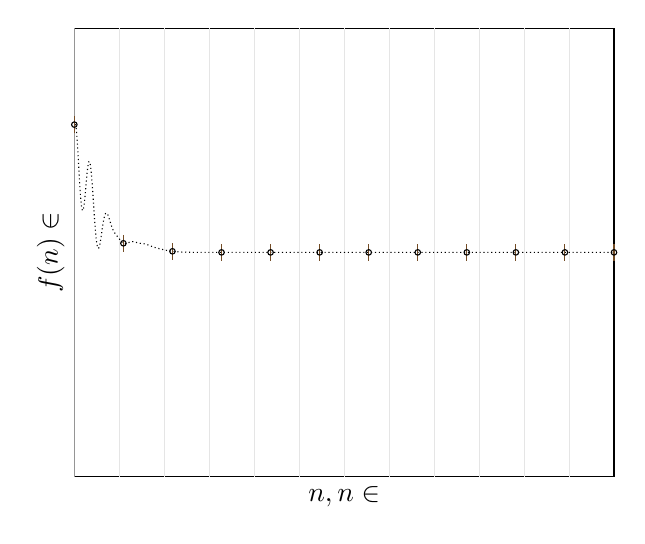
\begin{tikzpicture}
			\begin{axis} [
				xmin=\myxmin,xmax=\myxmax,
				ymin=\myymin,ymax=\myymax,
				xlabel={$n\sampletime, n \in \integers$},
				ylabel={$f(n\sampletime)  \in \realnumbers$},	
				xtick=\empty, 
				ytick=\empty, 
				]
				\foreach \i in {1, 2,...,\mynsamples}{
					\addplot[\mygridcolor, line width=0.1pt] coordinates {
						((\i-1)*\sampletimestep,\myymin) ((\i-1)*\sampletimestep,\myymax) 
					};
				}
				\addplot+[only marks, domain=\myxmin:\myxmax,samples=\mynsamples, mark color=\mycolor, mark=|, mark size=3pt, \mycolor]{\thefunction};
				\addplot+[only marks, domain=\myxmin:\myxmax,samples=\mynsamples, mark color=\mycolor, mark=o, mark size=1pt, mark options={fill=\mycolor, draw=\mycolor,}]{\thefunction};
				\addplot[domain=\myxmin:\myxmax,samples=1000, densely dotted, \mycolorii]{\thefunction};
			\end{axis}
		\end{tikzpicture}
	};	
	\node[anchor=center] (valdisc) at (0,-\myplotydist) {
		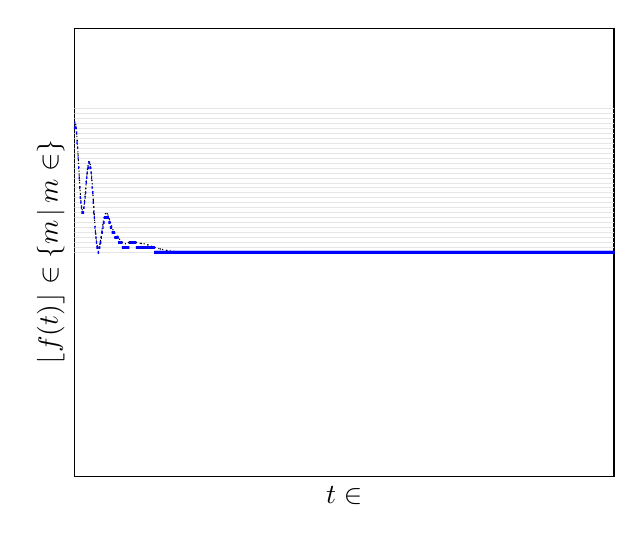
\begin{tikzpicture}
			\begin{axis} [
				xmin=\myxmin,xmax=\myxmax,
				ymin=\myymin,ymax=\myymax,
				xlabel= {$t  \in \realnumbers$},
				ylabel={$\lfloor f(t) \rfloor \in \{m\quantizestep \,\vert\, m \in \integers\}$},	
				xtick=\empty, 
				ytick=\empty, 
				]
				\foreach \i in {1, 2,...,\nquantsteps}{
					\addplot[\mygridcolor, line width=0.1pt] coordinates {
						(\myxmin, {(\i-1)*\quantizeres}) (\myxmax, {(\i-1)*\quantizeres}) 
					};
				}
				\addplot+[only marks,domain=\myxmin:\myxmax, samples=1001, \mycolor,mark=o,mark options={xscale=0.005, yscale=0.25}]{floor(\thefunction*\nquantsteps)/\nquantsteps};
				\addplot[domain=\myxmin:\myxmax,samples=1000, dotted, \mycolor]{\thefunction};
				\addplot[domain=\myxmin:\myxmax,samples=1000, densely dotted, \mycolorii]{\thefunction};
			\end{axis}
		\end{tikzpicture}
	};				
	\node[anchor=center] (timevaldisc) at (\myplotxdist,-\myplotydist) {
		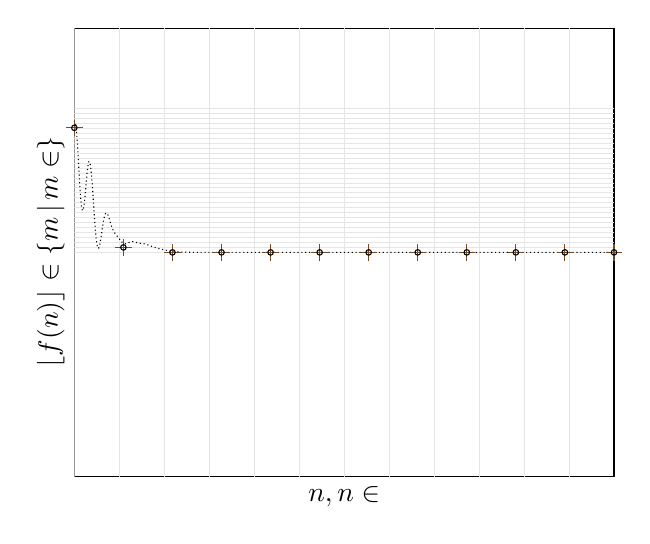
\begin{tikzpicture}
			\begin{axis} [
				xmin=\myxmin,xmax=\myxmax,
				ymin=\myymin,ymax=\myymax,
				xlabel= {$n\sampletime, n \in \integers$},
				ylabel={$\lfloor f(n\sampletime) \rfloor  \in \{m\quantizestep\,\vert\, m \in \integers\}$},	
				xtick=\empty, 
				ytick=\empty, 
				]
				\foreach \i in {1, 2,...,\nquantsteps}{
					\addplot[\mygridcolor, line width=0.1pt] coordinates {
						(\myxmin, {(\i-1)*\quantizeres}) (\myxmax, {(\i-1)*\quantizeres}) 
					};
				}
				\foreach \i in {1, 2,...,\mynsamples}{
					\addplot[\mygridcolor, line width=0.1pt] coordinates {
						((\i-1)*\sampletimestep,\myymin) ((\i-1)*\sampletimestep,\myymax) 
					};
				}
				\addplot+[only marks, domain=\myxmin:\myxmax,samples=\mynsamples, mark color=\mycolor, mark=+, mark size=3pt, \mycolor] {floor(\thefunction*\nquantsteps)/\nquantsteps};
				\addplot+[only marks, domain=\myxmin:\myxmax,samples=\mynsamples, mark color=\mycolor, mark=o, mark size=1pt, mark options={fill=\mycolor, draw=\mycolor,}]{floor(\thefunction*\nquantsteps)/\nquantsteps};
				\addplot[domain=\myxmin:\myxmax,samples=1000, densely dotted, \mycolorii]{\thefunction};
			\end{axis}
		\end{tikzpicture}
	};				
\end{tikzpicture}
	\caption{A visual overview about all pairings of discretization in time (sampling) and value (quantization).}\label{fig:discretization}
\end{figure*}
\clearpage

We consider \cref{fig:sampling} simply because it fits into the context of \cref{fig:discretization}.


\begin{myexample}[Aliasing]\label{exa:sampling}
	Let $f_0 = 0.125$. \cref{fig:sampling} shows three different signals
	\[
	\displaystyle f(t) = \cos(2\pi t f_0),\quad
	g(t) = \cos(2.5\pi t),\quad
	h(t) = \cos(1.75\pi t)
	\]
	 sampled with sampling frequency \(\samplingfreq=1\), \ie \(\samplingfreq = 1 = {1}/\sampletime\). $g$ and $h$ correspond to $\samplingfreq \pm f_0$.
\end{myexample}

\begin{figure*}
	\centering
	
\begin{tikzpicture}
	\def\myxmin{0}
	\def\myxmax{12}
	\def\myymin{-1.5}
	\def\sampfreq{1}
	\def\myymax{1.5}
	\def\mynsamples{12}
	\def\sampletimestep{1/\sampfreq}
	\def\mycolori{\colorforcurvesi}
	\def\mycolorii{\colorforcurvesv}
	\def\mycoloriii{\colorforcurvesii}
	\def\sigfreq{0.125}
	\def\thefunctionf{cos(deg((\sigfreq)*2*pi*x))}
	\def\thefunctiong{cos(deg((\sigfreq + 1*\sampfreq)*2*pi*x))}
	\def\thefunctionh{cos(deg((-\sigfreq + 1*\sampfreq)*2*pi*x))}
			\begin{axis}[
				width=\textwidth*0.8,
				height=5cm,
				xmin=\myxmin,xmax=\myxmax,
				ymin=\myymin,ymax=\myymax,	
				axis lines=center,	
				legend style={draw=none, at={(1.05,0.5)},anchor=west},
				xtick=\empty, ytick=\empty, 
				]
				\addplot[domain=\myxmin:\myxmax,samples=1000, \mycolori]{\thefunctionf};
				\addlegendentry{\(f(t)\)}
				\addplot[domain=\myxmin:\myxmax,samples=1000, \mycolorii]{\thefunctiong};
				\addlegendentry{\(g(t)\)}
				\addplot[domain=\myxmin:\myxmax,samples=1000, \mycoloriii]{\thefunctionh};
				\addlegendentry{\(h(t)\)}
				\addplot+[only marks, domain=\myxmin:\myxmax,samples=\mynsamples+1, mark color=\mycolori, mark=*, mark options={fill=\mycolori, draw=\mycolori,}]{\thefunctionf};
				\addlegendentry{\(f(n\sampletime)\)}
				\addplot+[only marks, domain=\myxmin:\myxmax,samples=\mynsamples+1, mark color=\mycolorii, mark=o, mark options={fill=\mycolorii, draw=\mycolorii,}]{\thefunctiong};
				\addlegendentry{\(g(n\sampletime)\)}
				\addplot+[only marks, domain=\myxmin:\myxmax,samples=\mynsamples+1, mark color=\mycoloriii, mark=-, mark options={fill=\mycoloriii, draw=\mycoloriii,}]{\thefunctiong};
				\addlegendentry{\(h(n\sampletime)\)}
				\foreach \i in {1, 2,...,\mynsamples}{
					\addplot[black!25, line width=0.1pt] coordinates {
						({(\i-1)*\sampletimestep},\myymin) ({(\i-1)*\sampletimestep},\myymax) 
					};
				}
			\end{axis}
\end{tikzpicture}
	\caption{\Cf \cref{exa:sampling}.}\label{fig:sampling}
\end{figure*}
